\section*{Motivation}

In this section we will describe the concept of multifunctionality and the relevance to the audience.

\subsection*{Biological Perspective of Neural Networks}
``A basic tenet of neuroscience is that the ability of the brain to produce complex behaviors such as sensory perception or motor control arises from the interconnection of neurons into networks or circuits.`` \cite{gettingEmergingPrinciplesGoverning1989}. 
Such networks have been a source of inspiration for \textit{artificial neural networks} (ANN). Similarly to a biological neuron, which ``\dots receives multiple signals through the synapses contacting its dendrites and sends a single stream of action potentials out through its axon\dots'', \cite{kriegeskorteNeuralNetworkModels2019}, an \textit{artifical neuron} is a unit that combines multiple inputs and provides a single discernible output. Such units can be combined in networks of arbitrary design. 
A sketch of a basic ANN is shown in Figure \ref{fig:neutral-network-diagram}.
\begin{figure}[!b]
    \begin{center}
    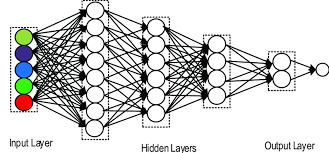
\includegraphics[scale=0.5]{Images/neutral-network-diagram.png}
    \caption{Sketch of an ANN with hidden layers, \cite{dumorEstimatingChinaTrade2019}}
    \label{fig:neutral-network-diagram}
    \end{center}
\end{figure}
Each layer's units connect to each of the next layer's units, and units themselves first calculate the linear combination of the inputs, and then perform a non-linear \textit{activation} on that linear combination. A network of this model, with at least one \textit{hidden} layer - i.e. a layer in between input and ouput layers, can be shown to be a \textit{universal approximator}, i.e. an algorithm that can approximate arbitrary functions, \cite{scarselliUniversalApproximationUsing1998}.

\subsection*{Biological Perspective of Multifunctionality}
We will follow \cite{flynnMultifunctionalityReservoirComputer2021a} in defining the multifunctionality as the networks ``...  of neurons whose activity patterns can change on the demand of performing a given duty, but synapses remain fixed.'' In other words, a multifunctional network can perform multiple tasks, without changing its inner structure. Such a definition is biologically motivated: even intuitively, we have a single brain which can both, say, write a poem and drive a bike. To be more specific, for example, \cite{briggmanImagingDedicatedMultifunctional2006} examined the neural activation of a medicinal leach when either crawling or swimming. The key finding was that the motions are driven both by multifunctional and dedicated circuitry. Even more interestingly, the overlap between neurons for the two motions is great: 93\% of the neurons that activated when swimming also activated when crawling. One of the proposed explanations is that ``...a single network driven at two different frequencies could generate motor patterns with different phase relationships without recruiting any additional neurons.'' (\cite{briggmanImagingDedicatedMultifunctional2006}). Furthermore, \cite{eschEvidenceSequentialDecision2002} showed that this switch in the behaviour happens according to the external stimuli, in this case the salinity level.
